%%%%%%%%%%%%%%%%%%%%%%%%%%%%%%%%%%%%%%%%%%%%%%%%%%%%%%%%%%%%%%%%%%%%%%%%%%%%%%%
% Chapter 'Refrigerants - R-410a'
%%%%%%%%%%%%%%%%%%%%%%%%%%%%%%%%%%%%%%%%%%%%%%%%%%%%%%%%%%%%%%%%%%%%%%%%%%%%%%%
\section{R-410a}
%
%%%%%%%%%%%%%%%%%%%%%%%%%%%%%%%%%%%%%%%%%%%%%%%%%%%%%%%%%%%%%%%%%%%%%%%%%%%%%%%
%%%%%%%%%%%%%%%%%%%%%%%%%%%%%%%%%%%%%%%%%%%%%%%%%%%%%%%%%%%%%%%%%%%%%%%%%%%%%%%
\subsection{Saturated Liquid Density - EoS1 - ID 1}
%
\begin{tabular}[l]{|lp{11.5cm}|}
\hline
\addlinespace

\textbf{Name:} & R-410a \\
\textbf{Equation:} & SaturatedLiquidDensity\_EoS1 \\
\textbf{ID:} & 1 \\
\textbf{Reference:} & Online: https://www.freon.com/en/-/media/files/freon/freon-410a-si-thermodynamic-properties.pdf?rev=6b72bfaa299142d697540982b88a56eb \\
\textbf{Comment:} & None \\

\addlinespace
\hline
\end{tabular}
\newline

\textbf{Equation and parameters:}
\newline
%
Saturated liquid density $\rho_\mathrm{sat}^\mathrm{liq}$ in $\si{\kilogram\per\cubic\meter}$ is calculated depending on temperature $T$ in $\si{\kelvin}$ by:
%
\begin{equation*}
\begin{split}
\rho_\mathrm{sat}^\mathrm{liq} &=& \begin{cases} \rho_\mathrm{ref} \exp(\Omega) & \quad \text{if flag } < 0 \\ \rho_\mathrm{ref} \Omega & \quad \text{else} \end{cases} & \quad\text{, with} \\
\Omega &=& \sum_{i=1}^{8} a_i \xi^{b_i} & \quad\text{, and} \\
\xi &=& 1 - \theta & \quad\text{, and} \\
\theta &=& \nicefrac{T}{T_\mathrm{crit}} & \quad\text{.}
\end{split}
\end{equation*}
%
The parameters of the equation are:
%
\begin{longtable}[l]{lll|lll}
\toprule
\addlinespace
\textbf{Par.} & \textbf{Unit} & \textbf{Value} &	\textbf{Par.} & \textbf{Unit} & \textbf{Value} \\
\addlinespace
\midrule
\endhead

\bottomrule
\endfoot
\bottomrule
\endlastfoot
\addlinespace

flag & - & 1.000000000e+00 & $b_4$ & - & 1.000000000e+00 \\
$T_\mathrm{crit}$ & $\si{\kelvin}$ & 3.452800000e+02 & $a_5$ & - & -7.171684000e-01 \\
$\rho_\mathrm{ref}$ & $\si{\kilogram\per\cubic\meter}$ & 4.889000000e+02 & $b_5$ & - & 1.333333333e+00 \\
$a_1$ & - & 1.000000000e+00 & $a_6$ & - & 0.000000000e+00 \\
$b_1$ & - & 0.000000000e+00 & $b_6$ & - & 0.000000000e+00 \\
$a_2$ & - & 1.984734000e+00 & $a_7$ & - & 0.000000000e+00 \\
$b_2$ & - & 3.333333333e-01 & $b_7$ & - & 0.000000000e+00 \\
$a_3$ & - & -1.767593000e-01 & $a_8$ & - & 0.000000000e+00 \\
$b_3$ & - & 6.666666667e-01 & $b_8$ & - & 0.000000000e+00 \\
$a_4$ & - & 1.819972000e+00 & & & \\

\addlinespace\end{longtable}

\textbf{Validity:}
\newline
Equation is approximately valid for $200.0 \si{\kelvin} \leq T \leq 345.28 \si{\kelvin}$.
\newline

\textbf{Visualization:}
%
\begin{figure}[!htp]
{\noindent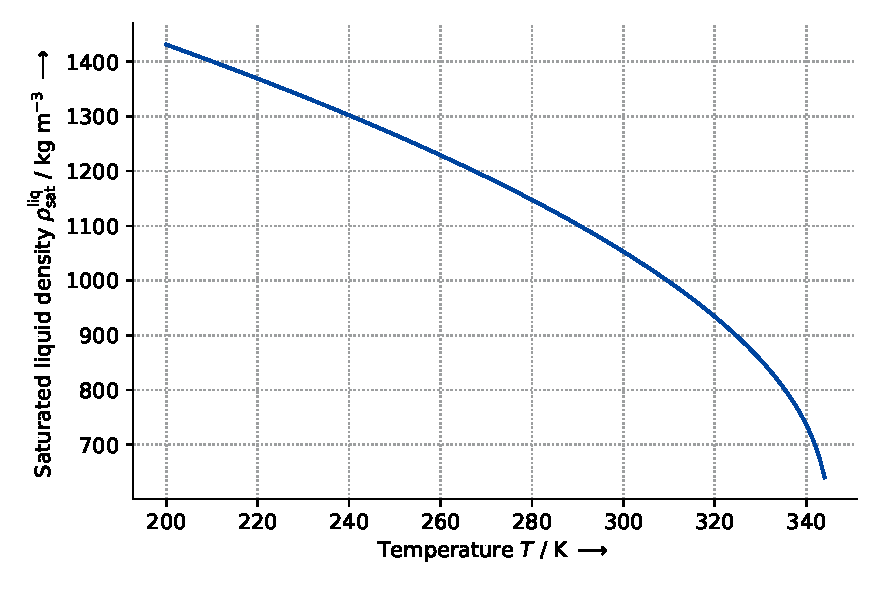
\includegraphics[height=10cm, keepaspectratio]{figs/ref/ref_R-410a_SaturatedLiquidDensity_EoS1_1.pdf}}
\end{figure}
%

\FloatBarrier
\newpage
%%%%%%%%%%%%%%%%%%%%%%%%%%%%%%%%%%%%%%%%%%%%%%%%%%%%%%%%%%%%%%%%%%%%%%%%%%%%%%%
%%%%%%%%%%%%%%%%%%%%%%%%%%%%%%%%%%%%%%%%%%%%%%%%%%%%%%%%%%%%%%%%%%%%%%%%%%%%%%%
\subsection{Vapor Pressure - EoS1 - ID 1}
%
\begin{tabular}[l]{|lp{11.5cm}|}
\hline
\addlinespace

\textbf{Name:} & R-410a \\
\textbf{Equation:} & VaporPressure\_EoS1 \\
\textbf{ID:} & 1 \\
\textbf{Reference:} & Lemmon, E. W. (2003): Pseudo-Pure Fluid Equations of State for the Refrigerant Blends R-410A, R-404A, R-507A, and R-407C. In: International Journal of Thermophysics 24 (4), S. 991–1006. DOI: 10.1023/A:1025048800563. \\
\textbf{Comment:} & None \\

\addlinespace
\hline
\end{tabular}
\newline

\textbf{Equation and parameters:}
\newline
%
Vapor pressure $p_\mathrm{sat}$ in $\si{\pascal}$ is calculated depending on temperature $T$ in $\si{\kelvin}$ by:
%
\begin{equation*}
\begin{split}
p_\mathrm{sat} &=& p_\mathrm{crit} \exp \left( \nicefrac{1}{\theta} \sum_{i=1}^{7} a_i \xi^{b_i} \right) & \quad\text{, and} \\
\xi &=& 1 - \theta & \quad\text{, and} \\
\theta &=& \nicefrac{T}{T_\mathrm{crit}} & \quad\text{.}
\end{split}
\end{equation*}
%
The parameters of the equation are:
%
\begin{longtable}[l]{lll|lll}
\toprule
\addlinespace
\textbf{Par.} & \textbf{Unit} & \textbf{Value} &	\textbf{Par.} & \textbf{Unit} & \textbf{Value} \\
\addlinespace
\midrule
\endhead

\bottomrule
\endfoot
\bottomrule
\endlastfoot
\addlinespace

$T_\mathrm{crit}$ & $\si{\kelvin}$ & 3.444940000e+02 & $a_4$ & - & -2.802200000e+00 \\
$p_\mathrm{crit}$ & $\si{\pascal}$ & 4.901200000e+06 & $b_4$ & - & 4.900000000e+00 \\
$a_1$ & - & -7.281800000e+00 & $a_5$ & - & 0.000000000e+00 \\
$b_1$ & - & 1.000000000e+00 & $b_5$ & - & 0.000000000e+00 \\
$a_2$ & - & 2.509300000e+00 & $a_6$ & - & 0.000000000e+00 \\
$b_2$ & - & 1.800000000e+00 & $b_6$ & - & 0.000000000e+00 \\
$a_3$ & - & -3.269500000e+00 & $a_7$ & - & 0.000000000e+00 \\
$b_3$ & - & 2.400000000e+00 & $b_7$ & - & 0.000000000e+00 \\

\addlinespace\end{longtable}

\textbf{Validity:}
\newline
Equation is approximately valid for $206.6964 \si{\kelvin} \leq T \leq 344.494 \si{\kelvin}$.
\newline

\textbf{Visualization:}
%
\begin{figure}[!htp]
{\noindent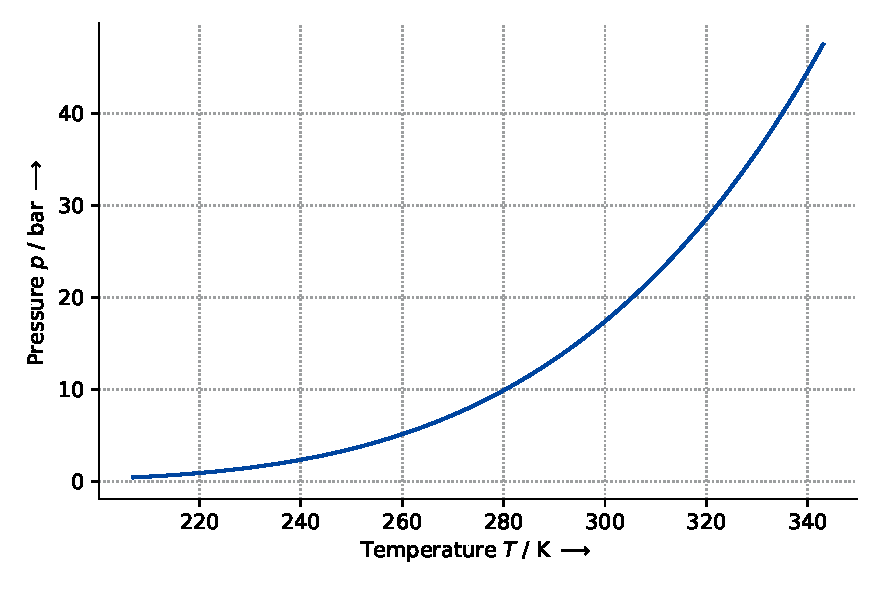
\includegraphics[height=10cm, keepaspectratio]{figs/ref/ref_R-410a_VaporPressure_EoS1_1.pdf}}
\end{figure}
%

\FloatBarrier
\newpage
%%%%%%%%%%%%%%%%%%%%%%%%%%%%%%%%%%%%%%%%%%%%%%%%%%%%%%%%%%%%%%%%%%%%%%%%%%%%%%%
